\chapter{Grundlagen}

\section{Computational Thinking}

Unter Computational Thinking (CT) wird Kognitionsprozess oder Gedankenprozess verstanden, der durch
die Fähigkeit, in Form von Dekomposition, abstrahierend, evaluierend, algorithmisch und
generalisierend zu denken, reflektiert wird \cite{selby_computational}. Nach \cite{wing2011research}
ist Ziel des Prozesses, ein Problem so darzustellen, dass es von einem Computer gelöst werden kann.  
Dazu werden zur Entwicklung von Problemlösungen logische Artefakte erstellt, die auf dem Computer
ausgeführt werden. Dies kann zum Beispiel Quelltext in einer Programmiersprache sein.

Diese Arbeit fokussiert sich primär auf algorithmisches Denken, Abstraktionen und Evaluation.
Algorithmisches Denken beschreibt die Fähigkeit, ein Problem sequentiell abzuarbeiten. Dazu werden
Kontrollstrukturen als Teil eines Abstraktionsprozesses genutzt. Um zum Beispiel eine Wiederholung
eines Befehls umsetzen, könnte der Befehl mehrfach hintereinander im Quellcode stehen. Zur
Komprimierung des Codes kann man die Wiederholung mit einer Schleife abstrahiert werden. Dazu muss
ein zusätzliches Vokabular verwendet werden, dass dem Computer klar macht, dass dieser Befehl
mehrfach wiederholt werden soll. Eine tiefere Abstraktion kann an diesem Beispiel erfolgen, wenn
durch die Nutzung von Variablen innerhalb der Schleife mit jeder Wiederholung unterschiedliche Werte
benutzt werden. Ein weiteres abstrahierendes Konzept besteht darin Prozeduren und Funktionen zu
bilden. Dabei werden mehrere Kommandos werden unter einem Namen gebündelt und parametrisiert, und im
Fall von Funktionen ein Rückgabewert generiert. Prozeduren und Funktionen können mehrmals an
verschiedenen Stellen im Programm aufgerufen werden zu können, ohne die Kommandos einzeln zu
wiederholen. Abstraktionen erlauben uns Konzepte auf einer Metaebene zu nutzen und diese dann
umzusetzen.

Zur Entwicklung der logischen Artefakte gehört neben der Programmierung selbst auch die Evaluation
des Artefakts. Dazu wird es ausgeführt und anschließend mithilfe von visuellen oder textuellen
Feedback analysiert. Aufgrund des Feedbacks werden Rückschlüsse darüber gezogen, ob das zugrunde
liegende Problem gelöst wurde, und wenn nicht, wie das Artefakt verändert werden muss, um das
Problem adäquat zu lösen.

In einer Richtlinie zur Etablierung von Computational Thinking in der K-12-Bildung
(\cite{leadership_toolkit}) der International Society for Technology in Education und Computer
Science Teacher Association wird die Wichtigkeit von CT beschrieben: \em \enquote{Because we can
expect that every student will rely on computing in some way to amplify his or her skills, we must
ensure that all students have the opportunity to learn the basics of CT during their K–12
education.} \em.

\section{Turtle Geometrie}

Den Computer als Werkzeug zum Lernen zu benutzen ist der Fokus von Seymour Paperts Forschung zu Logo
und der Turtle-Umgebung \cite{papert1980mindstorms}. Logo ist eine Programmiersprache die dazu
gestaltet ist, möglichst einfach zu erlernen zu sein. Dazu besitzt sie eine minimale Syntax und ein
minimales Kontingent an Kontrollstrukturen.

Papert konzipiert die Turtle-Umgebung zur Exploration mathematischer Konzepte. Sie ist ein Beispiel
einer Mikrowelt, eine Anwendung in der Objekte programmatisch manipuliert werden können, um dem
Lerner ein Medium zu bieten, dass dem natürlichen Erlernen eines Konzepts dient. Die Turtle ist ein
Objekt, das mithilfe von einfachen Kommandos bewegt werden kann. Durch Aktivierung eines Stifts wird
die Ausgabe von Linien erzeugt, die der Bewegung folgen. Die Bewegung der Turtle erfolgt mittels
Logo-Programmen.

Papert argumentiert, dass eine Mikrowelt dann zum einem wertvollen Lerninstrument wird, wenn sie dem
eine natürliche Interaktion erlaubt. Die Bewegung der Turtle soll dem Sprechen mit der Turtle
gleichen. Die Definition von Prozeduren gleicht dem Beibringen eines neuen Vokabulars. Das Erlenen
eines Konzepts wird dann durch iteratives Vorgehen ermöglicht, dass der Exploration und dem Lernen
einer der menschlichen Sprache im Kindesalter gleicht. Das Objekt, dass in der Mikrowelt manipuliert
wird, sollte dabei menschliche Charakteristiken besitzen. Die Turtle ist \enquote{body-syntonic},
ihre Bewegung und Orientierung lässt sich konkret auf die Bewegung und Orientierung des Menschen
übertragen. Um das Verhalten der Turtle nachzuvollziehen, kann der Lerner den eigenen Körper als
Referenz nutzen.


\section{Game-based learning von Computational Thinking}

Spiele werden häufig dazu genutzt, als Lernumgebungen zum Erlenen von Computational
Thinking-Konzepten zu dienen (z.B. \enquote{Program your Robot} \cite{kazimoglu_serious_2012},
\enquote{Lightbot} \cite{gouws2013computational} oder AgentSheets \cite{repenning2010scalable}). Diese Lernumgebungen zeichnen sich dadurch aus, dass sie Computational Thinking-Fähigkeiten direkt auf Spielelemente mappen. Zusätzlich können Spiele aufgrund der Herausforderung, die sie stellen, einem Fantasieaspekt der den Lerner in
eine imaginäre Welt versetzt, dem Ausnutzen der natürlichen menschlichen Neugierde, und der
Kontrolle, die der Lernen über den Spielverlauf zu geben, Mikrowelten in einer Weise bereit stellen,
in der Lerner internal motiviert sind Spielziele zu verfolgen und damit Lernerfolge zu erzielen
(\cite{rieber_seriously_1996}).

\subsection{RoboCode}

RoboCode\footnote{https://sourceforge.net/projects/robocode/} ist ein Spiel, dass zum Erlernen der
Programmiersprache Java konzipiert wurde. In einer Arena (Abb. \ref{robocode}) versuchen zwei oder mehrere Roboter sich
gegenseitig zu zerstören. Dabei führen die Roboter Kampfstrategien in Form von Java-Programmen aus.
RoboCode integriert einen Quellcode-Editor, in dem diese Strategien gebaut werden können.
Mitgelieferte Beispielstrategien können als Orientierung dienen und als Gegnerstrategien festgelegt
werden.

\begin{figure}
  \caption{Ein Kampf zwischen zwei Robotern in RoboCode.}

  \label{robocode}
  
  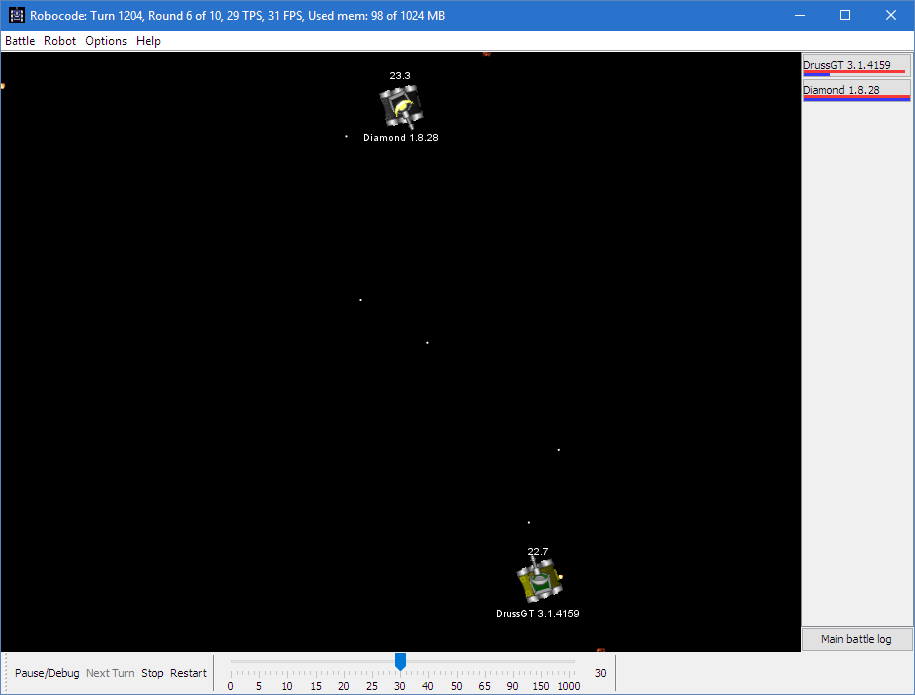
\includegraphics{figures/RoboCode.png}
\end{figure}

Um RoboCode hat sich eine Community gebildet. Im
RoboCode-Wiki\footnote{http://www.robowiki.net/wiki/Robocode} enthält eine Dokumentation des Spiels,
Anleitungen zum Erstellen eigener Strategien, und weitere Kampfstrategien zum Download.
RoboRumble\footnote{http://literumble.appspot.com/} ist eine Sammlung von dauerhaft aktualisierenden
Ranglisten, in denen von Spielern hochgeladenene Kampfstrategien aufgrund von Kämpfen gegeneinander
eingestuft werden. Die Strategien können heruntergeladen, eingesehen und für eigene Kämpfe benutzt
werden.

\subsection{ctGameStudio}

CTGameStudio (\cite{werneburg_ctgamestudiogame-based_2018}) ist eine webbasierte Spielumgebung zum
Erlernen von CT-Fähigkeiten und Programmierung. Mithilfe eines Editors entwickeln Schüler ein
Programm zur Steuerung eines virtuellen Roboters in einer Mikrowelt.

Der Editor ist ein visuelles, blockbasiertes Programmierwerkzeug basierend auf der
Blockly-Bibliothek\footnote{https://developers.google.com/blockly/}. Visuelle blockbasierte Editoren
haben sich als einsteigerfreundliche Programmierwerkzeuge erwiesen (\cite{weintrop_block_2015}).
Programmkonstrukte werden durch Blöcke repräsentiert, die mittels Drag-and-Drop ineinander
verschachtelt und kombiniert werden, um ein Programm zu bilden. Eine Blockbibliothek gibt eine
eingebaute Übersicht über die verfügbaren Programmkonstrukte, so dass auf einen Blick die
Möglichkeiten der Programmierung eingesehen werden können. Durch die strukturierte Komposition von
Blöcken können keine Syntaxfehler auftreten, was in textbasierten Programmen eine häufige, den
Spielfluss störende Fehlerquelle ist.

Zur Einführung in die Programmierung und Vermittlung von CT-Fähigkeiten, sowie zur Einführung in die
Mechaniken des Spiels enthält das ctGameStudio einen Storymodus. Der Storymodus enthält mehrere
Level, die nacheinander abgearbeitet werden, und jeweils auf das Erlenen einer oder mehreren
CT-Fähigkeiten, einer neuen Abstraktion oder Roboterfähigkeit abzielen. Dazu enthält das Level eine
Aufgabenbeschreibung, Anleitungen und optionale Hilfestellungen. Zur Lösung eines Levels baut der Schüler ein
Programm welches einen Algorithmus darstellt, der den Roboter so steuert, dass die Herausforderung
gelöst wrid. Diese Problemlösungstrategie kann immer wieder neu ausgeführt werden, bis das
gewünschte Ziel erreicht wurde. Ist das der Fall, wird zum nächsten Level fortgeschritten. Mit
steigenden Level erhöht sich die Komplexität der benötigten Lösungstrategien. So reicht im ersten
Level ein einfacher Befehlsaufruf, während im letzen Level durch gezielte Bewegung, Zielen und
Schießen ein Gegner besiegt werden, bevor dieser einem zu viel Schaden zufügt.

Angelehnt an der Turtle-Geometrie nach Papert wurde eine Bewegungssemantik für den Roboter
entwickelt, und um Fähigkeiten erweitert, die für die das Spielen der Story relevant sind.

\begin{itemize}
\item Positionierung auf dem Spielfeld durch die Bewegung um eine Distanz oder bis zu einem Punkt
auf der x- und y-Achse, der Bewegung bis die Spielfeldgrenze, ein Gegenstand oder der Gegner berührt wurde, dem Drehen um einen
Winkel, und dem Drehen, um einen Punkt anzupeilen.
\item Angriff durch Abgeben eines Schusses in Blickrichtung.
\item Das Ausfinden machen des nächstgelegenden Objektes oder Gegners durch einen Scanvorgang in eine Richtung. Wurde
  ein Ergebnis gefunden, kann die Distanz und Winkel zum Ergebnis und seine Position gelesen werden.
\item Feststellen von Ereignissen, wie der Fall ob man getroffen wurde, oder ob man mit der Wand,
  einem Gegner oder einem Objekt kollidiert ist.
\item Lesen der eigenen Attribute, darunter die Position auf dem Spielfeld und die Anzahl an
verbleibenden Lebenspunkten.
\end{itemize}

Nach Beenden des letzten Levels sind die Inhalte des ctGameStudio im aktuellen Stand ausgeschöpft.
Dabei wäre es sinnvoll, Schülern eine Möglichkeit zu geben, ihre gelernten Fähigkeiten anzuwenden.
Während Schüler im Storymodus konkrete Anweisungen zu der Lösung eines Problems bekommen, sollte das
Spiel Herausforderungen enthalten, die eigenständig vom Schüler gelöst werden müssen, um besonders
die Evaluationsfähigkeit stärker auszubilden. Spiele wie RoboCode zeigen uns, dass ein Spiel durch
einen offenen Spielmodus einen hoher Wiederspielwert erreicht werden kann.
